% !TEX root = ../main.tex
\chapter{Background}

The purpose of this work is to efficiently make use of multiple threads with the LowLevelAnalyzer (LoLA).

%TODO: separate chapter?
Lolas development startet in 1998. It was aimed to be used by third party tools to check properties of petri nets \cite{schmidt2000lola}. Since then it was steadily updated to compete with other state of the art tools. Recurring prizes in a model checking contest with focus on petri nets suggest a success in this attempt \cite{MCC2017}.
The internal property evaluation however, is still most performant single threaded. To evaluate a property of a petri net, LoLA searches all necessary net states that can be reached from the initial one. The search is a depth first search on an undirected graph. The graph is discovered during the search itself.

Parallelization of depth first search is a difficult matter. Although rather general algorithms exist (some of them mentioned in the previous chapter), they usually make use of an assumption which cannot be made with LoLA.%TODO: reference dfs correctly

For the quite specialized search in LoLA, a previous attempt of parallelization exists. Unfortunately the performance is usually worse then the single threaded approach. It even gets worse the more threads are used.

This is the staring point of this work. There is an algorithm which is not performing as expected. The most important task, is to find the bottle neck of this algorithm. After that it is desired to remove that bottleneck. The improved version should hopefully outperform the single threaded algorithm with use of a reasonable amount of threads. Additionally a desirable result would show a linear (or better) scaling of the performance with the amount of threads.

\section{Performance Measurement}
\label{benchmarking}
\subsection{A distinction between different views on software}
The performance of a program is a property which is always of interest somehow. Even if it is not a critical aspect in the working environment. But as reachable the concept of performance might look at first, the complicated it can get.

Just like that, what is called a performant application is highly dependent on its environment. The possibly most obvious characteristic would be the time it takes to execute a program or a subroutine. But in a lot of szenarios, the time consumption actually does not matter that much. A user might not even notice a factor of 1000 between routines that operate in an order of micro seconds. At the same time he might worry that the program can access enough memory to finish its task. That means before measuring the performance of a program or subroutine, one must define the characteristics that define the performance of exactly that given program or subroutine. Other characteristics beside execution time and memory consumption can be network latency, energy consumption or responsibility. Ultimately it is everything that increases the useability of a program.

After knowing what will be measured the reasonable next concern is how it will be measured. The act of measuring is typically called benchmark and the approach here is influenced by the scope of the measurement. Oaks describes a general distinction between macro, meso and micro benchmarks \cite{oaks2014java}. Each type addresses a different scope of a programm.%TODO: don't address oaks directly

Macro benchmarks give an overview over the entire execution. The data collection is often less complicated since it is done over the whole application runtime and hardly requires any modifications to it. Measuring the runtime of a program is as simple as it gets: the difference between the end and the start of the program. The memory allocation can often also be measured with simple tools that the operating system or other third party software provide. The downside is that a lot of software cannot be measured at all in this scope. So it is a property of event driven programs that they do not terminate at a known point in time and therefore the execution time is of limited use.

Micro benchmarks consider the most narrow aspects of an application. They messure the execution of single instructions or atomic routines. Results of micro benchmarks have to be taken with a grain of salt because compile and hardware optimization strongly influences the results. Assumptions that work for the single code snippet might become false after the compiler integrates that part into the complete program or vise versa. It is a good advise to use a benchmarking tool which is built for this task. Overwise there is a risk to be trapped in false results. Like compilers that are optimizing away whole loops (which in turn often be the benchmark itself), because the result can be evaluated at compile time. The advantages of micro benchmarks however, is that different implementations of basic algorithms can be compared directly. Provided they are performing equivalent in the macro scope of the program.

After the previous scopes described a detailed view and an overview, the last scope has to be something in between. And this holds true for the so called meso benchmark. Perhaps the best explanation for this kind is, that a meso benchmark is what is not macro nor micro benchmark. Meso benchmarks deal with parts of a program that get more complex. Like Modules or further reaching subroutines. These can be the most interesting benchmarks since they can narrow down bottle necks to specific parts of the software. Unfortunately they often require to manipulate the program in some way. Which again means that the measured performance differs from the actual performance.


\subsection{Methods of measurement}
\label{BenchMethods}
For the actual measurements, two basic approaches can be distinguished: manual implementation or usage of a tool.

The quickest and most precise approach is to make own measurements. Self written, and therefore known software can be easily extended e.g. by counters for variables or measurements of time periods. All measurements can be tailored to the individual use case and results can be exported in the most convenient format. On the over hand this approach can come with several downsides. Some of them might be that the maintenance of the measurements can get increasingly complex the more numerous they get, added code will influence the performance of the software itself, and own mistakes might hide behind satisfying results. And there are probably other reasons that can be thought of, but short, temporary measurements of this kind might give o quick overview the own software.

Probably the safer approach is the usage of a tool. There exist a variety of tools which are build for the inherent purpose to measure application performance with common metrics and use cases. Since the metrics reflect some characteristics of an application - a profile - these tools are typically called profilers. Using established profilers for performance measurement can help avoiding common traps and mistakes especially when they were designed by experienced developers who are skilled in this area. But it also means to invest time and effort to learn how to use it and how to interpret its results.

Profilers aid to do the things automatically that otherwise would have to be implemented manually. An often used method to figure out bottle necks is to take samples of the call stack during program execution. The calls that are most frequently sampled will correlate with the program parts where the most time was spent in. Another method is to use code injections. Here, code is inserted automatically into the source or binary code at relevant spots. The injections are then used to count events or measure time intervals.

With the general techniques in mind we can proceed to the actual software and its characteristics that will be examined in this work.

\section{Implementation Details}
\subsection{Code Base}
This work is based on a previous attempt by Gregor Behnke to use multiple threads for LoLA. For this reason, his code will be taken as base implementation for the parallel search. In the LoLA project structure, this would correspond to the \texttt{ParallelExploration} class in src/Exploration.

This class itself seems to be based on a single threaded algorithm in the \texttt{DFSExploration} class, since the basic structure and several lines of code as well as comments are equivalent. The base algorithm was then altered by Behnke to make data manipulation thread safe. This implies that no specialized Depth First Search algorithm was used, but the existing algorithm was extended.

The purpose of the exploration class family in LoLA, is to keep track of the \textbf{paths} that where discovered during the search. The actual net \textbf{states} that are the vertices of the path, are managed by another family of classes: the store classes. In more detail this means that the exploration class will store the edges that lead to the current net state and choses which edges of the graph will be used next to discover another net state. The discovered net states will be handed to the store class. It will tell the exploration class if this net state was already discovered earlier. If that is not the case the net state will be stored permanently

Behnke tried to implement multi threading (inside the exploration class) by exploring a different path with each thread. He therefore introduced thread local variables that keep track of the path, determine which edge will be expanded next and what the current net state is. The store is globally shared. Thread safe searching and adding to the store must be implemented by the store itself for this approach. The crucial work of Behnke inside the exploration algorithm, was to distribute the work over all threads and keep the data synchronized.

Load distribution is done with a simple approach. If a thread can expand multiple edges and an idle thread exists, one edge will be discovered by the current thread and another will be discovered by the next possible idle thread. The data will be synchronized, so that the woken up thread will copy the previously discovered path of the waken. Cases like: what should be done if a thread has no more work (accessible edges) left or what to do if the current net state satisfies the asked property, are also handled.

The store which is used by LoLA in the default case (\texttt{PluginStore}) does not provide any thread safety. The thread number is completely ignored within the relevant parts and so the behavior of this store when using multiple threads is undefined. But there is another store implementation which implements several buckets to store the states in: the \texttt{HashingWrapperStore}. The buckets should only be accessible by at most one thread. The net states that should be stored are now given a hash value and every bucket has a range of hash values associated with them. With this solution multiple searches can be issued, as long as the hash value of the searched net states differ.

The actual classes which are used at runtime to expand the search tree, are determent by the call switches which are handed to the LoLA executable. The relevant switches for the parallel exploration are \texttt{--threads=[threadCount]} and \texttt{--bucketing=[bucketCount]}. A thread count greater then 1 will tell LoLA to use the \texttt{ParallelExploration} class and the bucketing switch will signal to use a hashing store.

\subsection{Data Synchronization}
To keep global data consistent, a method is needed to synchronize this kind of data between threads. A common way to achieve this, is to restrict the access to one thread at a time. for this the concept of mutexes and semaphores are often used as locks for access control. The downside of this approach is a bottleneck at this global data. If access is granted to at most one thread, every calculation that is done while accessing, is also done at most with the speed that a single thread can provide. Therefore accessing this regions (including locking and unlocking them) should be done as infrequent and as quick as possible.

Since LoLA computes a lot of short and low level instructions, locking and unlocking data segments might sum up to a significant amount of time. So the locking mechanism used by LoLA might also be a good starting point to search for a reason for that unexpected performance that LoLA shows.

Behnke used locks from the pthread library \cite{?}. A possible substitute would be an own implementation with a Compare And Swap instruction as spin lock. This has the potential to keep the overhead for the locks at a bare minimum.

\section{Environment}
\label{env}
The used development environment consist of two machines. The general development is done on a virtual machine (vm). It runs with 4 threads on a Intel(R) Core(TM) i7-4770S CPU @ 3.10GHz with 4 physical cores. Each core supports hyper threading which makes a sum of 8 threads on the host of the vm. A total of 17.4 GB of physical memory is available for use inside the vm. Ubuntu 4.10 is running as operating system.

As a performant testsystem a powerful server (ebro) was used. Ebro has 4 AMD Opteron(tm) 6284 SE processors. Each with 16 cores and 2.7GHz base clock with a max boost of 3.4GHz \cite{AMDSpecs}. This sums up to 64 physical cpu cores (and threads) in total. As physical memory 995.2 GHz are installed. The operating system is CentOS Linux 7 Core (collected with hostnamectl command).

If no other source is provided the data was collected with the proc filesystem provided by the linux distributions.
\begin{center}
    \begin{table}[H]
        \centering
        \begin{tabular}{ | l | c | c |}
            \hline
            \textbf{Spec Name} & \textbf{VM} & \textbf{Ebro} \\ \hline
            Max. Clock per Thread & 3.1GHz & 3.4GHz \\ 
            Available Threads & 4 & 64 \\ 
            Memory & 17.4 GB & 995.2 GB\\ 
            Operating System & Ubuntu 4.10 & CentOS 7 Core \\ \hline
        \end{tabular}
        \caption{Specifications of the two development systems}
    \end{table}
\end{center}

% - ebro\\
% model name      : AMD Opteron(tm) Processor 6284 SE
% cpu MHz         : 1400.000
% 4 cpus 16 cores 16 threads
% MemTotal:       1043610248 kB

% - vm\\
% model name      : Intel(R) Core(TM) i7-4770S CPU @ 3.10GHz
% cpu MHz         : 3100.006
% MemTotal:       18281952 kB
% SwapTotal:       2097148 kB

\chapter{Approach}
%TODO:
% was erwartet mich in diesem kaitel
% warum bin ich so vorgegangen
% was wird am ende stehen (ohne genaue werte)
% wo können referenzen gefunden werden? http://www.cplusplus.com

\section{Switching The Synchronization}
The first step taken was switching from the pthread library to a compare and swap (CAS) algorithm. Since C++ 11 there is an equivalent implementation in the standard library called \texttt{bool std::atomic::compare\_exchange\_weak(T\& expected, T val)} (or \texttt{bool std::atomic::compare\_exchange\_strong(T\& expected, T val)}) that was used for this task. This function compares the current value of an \texttt{std::atomic} with \texttt{expected} and replace it with \texttt{val} if the comparison returns true. If it returns false it replaces \texttt{expected} with the actual value of the atomic. The weak version is allowed to return false in favor for a general performance gain, even if the compared values are actually equal.

To represent a lock that can either be locked or unlocked, a boolean as value is sufficient. To shape a spin lock like mutexes and semaphores with a CAS function, they have to loop until the expected value compares equal. There are two reasonable modes to lock: the first is to just wait until an observed lock is unlocked and the second is to wait for an unlock with an immediate locking. The first approach can be helpful to suspend the execution of the current thread until an external thread is signalling a continuation. The second approach can be used to block access to a resource until all preceeding manipulations are completed. At last there are functions necessary that can block or release the resource in a privileged manner. The resulting implementation is shown in listing \ref{CASIMPL}.

Swapping the old pthread implementation with the new CAS implementation now remains a matter of search and replace. The equivalent of the mutexes \texttt{pthread\_mutex\_lock()} is \texttt{waitAndLock()}. \texttt{Pthread\_mutex\_unlock()} corresponds to \texttt{unlock()}. The previous \texttt{sem\_wait()} correspond to a \texttt{waitForUnlock()} call after a \texttt{lock()}. And \texttt{sem\_post()} corresponds to \texttt{unlock()}.\\
However, this is a very specialized replacement which acts as a proof of concept. Other parts of the code might have to be replaced in another way, depending on the semantics of the part. Additionally the CAS implementation is as short as possible. The pthread library comes with some importend features like a mechanism to reduces the risk of dead locks and different modes for the semaphores.

\lstset{language=C++,caption={Basic implementation of a spin lock with compare and swap},label=CASIMPL, frame=none, stepnumber=5, backgroundcolor=\color{verylightgray}}
\begin{lstlisting}
#include <atomic>

enum LOCK{
    LOCKED,
    UNLOCKED
};

static inline void waitAndLock(std::atomic<bool>* lock){
    bool expected = UNLOCKED;
    while (!lock->compare_exchange_weak(expected,LOCKED)){
        expected = UNLOCKED;
    }
}

static inline void waitForUnlock(std::atomic<bool>* lock){
    while (lock->load() != UNLOCKED){
        continue;
    }
}

static inline void lock(std::atomic<bool>* lock){
    lock->store(LOCKED);
}

static inline void unlock(std::atomic<bool>* lock){
    lock->store(UNLOCKED);
}
\end{lstlisting}

\section{Finding the bottleneck}
\subsection{Benchmark characteristics}
We have now an application with a bottleneck and a possible solution to fix that bottleneck. Next we will compare the performances.

In this case, performance means execution time. The expectation is that the execution time decreases with an increased amount of threads (computing power). The time is therefore the characteristic of interest.

As test systems the both machines described in \ref{env} where used.

As test data a predefined petrinet of the dining philosophers was used. It is a common concept in theoretical computer science to illustrate problems and risks of parallel processes and was originally introduced by Dijkstra \cite{dijkstra1971hierarchical}. The philosophers count can be scaled to an arbitrary amount. This is useful to increase the complexity (and therefore the execution time) of the net to a convenient level. The reachability graph is also reasonably branched to allow a parallel discovery. The actual used net is a version with one thousand philosophers.
%TODO: reachability graph of dining philosophers

LoLA is executed with the \texttt{--threads=[threadCount]} and \texttt{--check=full} switches. The first switch simply sets the amount of threads that should be used for the state exploration. The second switch cause LoLA to explore the whole state space without exploring a property. This ensures that the application will terminate after all states have been discovered and no varying discovery paths can influence the execution time.

\subsection{A general performance survey}
LoLA will spend most of the time inside the depth first search of the state exploration. For this reason a simple execution with the given parameters will uncover if the different synchronization implementations have an impact on the performance. This would correspond to the macro benchmark scope and can be achieved without any additional modification or tools because LoLA already measures its own execution time.

Unfortunately a simple testrun on the VM reveals that there is no performance gain. Figure TODO:ref shows that the new implementation is actually slower than the previous. But as stated in TODO:ref, the performance of the original implementation always stayed behind the sequential algorithm. This means that a relevant speedup would divide the execution time by an order of the used threads. Taking this expectation as base, both implementations still can be considered in the same order of performance. Thus, we can conclude that we either missed the cause of the bottleneck, or the new implementation faces similar challenges.

%TODO: fix diagram, add label
\begin{figure}
\centering
\begin{tikzpicture}
    \begin{axis}[
        width=0.9\textwidth, 
        height=0.3\textheight,
        xbar, axis on top,
        xmajorgrids=true,
        bar width=16,
        title={Macro Benchmark},
        xtick={0,50,100,150,200,250,300},
        xmin=0,
        x tick label style={/pgf/number format/1000 sep=},
        xlabel={seconds},
        ytick={1,2},
        yticklabels={PThread,CAS},
        y tick label style={/pgf/number format/1000 sep=},
        bar shift=0,
        enlarge y limits=1,
        nodes near coords,
        nodes near coords align={horizontal},
        %
        legend style={
            at={(0.5,-0.15)},
            anchor=north,
            legend columns=-1,
            /tikz/every even column/.append style={column sep=0.5cm}
        }
        ]

        \addplot table [x=master-t1-b0, y expr=1, col sep=comma,trim cells=true] {data/allMacroData.csv};
        \addplot table [x=atomics-t1-b0, y expr=2, col sep=comma,trim cells=true] {data/allMacroData.csv};
        \legend{PThread, Compare And Swap}
    \end{axis}
\end{tikzpicture}
\caption{Macro benchmark comparison between the original (PThread) implementation and the substitute (Compare and swap)\\ LoLA call: "lola --check=full --threads=4 ../tests/testfiles/phils1000.lola" }
\end{figure}

\begin{center}
    \begin{table}[H]
        \centering
        \begin{tabular}{| c | c |}
            \hline
            \textbf{PThread} & \textbf{Compare And Swap} \\ \hline
            262s & 274s \\ \hline
        \end{tabular}
        \caption{Macro benchmark comparison between the original (PThread) implementation and the substitute (Compare and swap)\\ LoLA call: "lola --check=full --threads=4 ../tests/testfiles/phils1000.lola" }
    \end{table}
\end{center}

The benchmark result shows no significant change in performance. Therefore an exhaustive evaluation with multiple testruns is dropped in favor of a detailed bottle neck analysis. In the next section we will use a more precise benchmark method to inspect the search characteristics.

\subsection{Searching for inefficient application components}
To develop a deeper understanding of the internal processes, we have to examine the individual program parts. The most important one remains the search for net states which is done in the \texttt{ParallelExploration} class.

LoLA will call the \texttt{depth\_first()} method of the \texttt{ParallelExploration} to initiate the search. There, all search threads will be initialized, started and destroyed (after they finished their work). Starting and destroying the threads takes constant time per thread. Since we will work with very few threads in relation to the amount of states we will handle, these parts are insignificant for the performance measurement and can be ignored. But each thread will execute the \texttt{threadedExploration} method. This method is the algorithm for the actual search. It will loop until a given predicate is satisfied by any thread. For these reasons we will focus our measurements on this method.

We now know a precise code section that we want to inspect. Next we have to choose a new measurement method. We can decide between two general approaches: we can use an existing tool that can hopefully inspect the application parts we are interested in, or we can extend our code manually. Both approaches have their up and downsides. In our case we decided to use the manual approach. First because the interesting code is relatively short and clear and second because it can be done right away, without spending much time for learning a third party software.

In the next step measurements have to be inserted at the relevant sections. However, what section is relevant cannot be known before measuring. We have to choose parts that seem to be most likely. This is an inherently subjective process, but some factors will be influential. For example, elemental assignments like \texttt{x = 5;} will take an insignificant amount of time, whereas function calls and loops can take arbitrarily long times to be executed. The cost of a bad selection is very low, since the measurements can be easily changed in the short method.

The time was measured with the functions provided by \texttt{std::chrono} from the c++ standard library. The exact code is considered trivial and will not be discussed further.

Table TODO:ref is listing the performance of the code pieces that are considered relevant. Over less important measurements are omitted to keep a clear view. Here is an explanation of the values:
\begin{itemize}
    \item Total Thread Time - The cumulative time spend in each thread is called total thread time.
    \item Synchronization Time - Time spend to synchronize the threads with mutexes.
    \item Store Search Time - Time spend inside the \texttt{searchAndInsert} call. A method to safe the discovered states.
    \item Idle Time - The Time each thread spent for the \texttt{restartSemaphore} to be unlocked
    \item Work - Time that each thread spend while having states left that can be discovered
    \item No Work - Time spend during waiting for new states that can be expanded including reinitialization. 'Work' and  'No Work' should cover the complete search loop.
\end{itemize}

\begin{center}
    \begin{table}[H]
        \centering
        \begin{tabular}{ | l | c | c | c | c |}
            \hline
            \textbf{} & \textbf{Trhead 0} & \textbf{Trhead 1} & \textbf{Trhead 2} & \textbf{Trhead 3}\\ \hline
            Total Thread Time & 256s & 256s & 256s & 256s \\ 
            Synchronization Time & 0.00000004s & 0.00000004s & 0.00000005s & 0.00000005s \\
            Store Search Time & 58s & 58s & 56s & 58s \\ 
            Idle Time & 0.22s & 0.22s & 0.22s & 0.22s \\ 
            Work & 64s & 64s & 62s & 64s \\ 
            No Work & 0.5s & 0.5s & 0.5s & 0.5s \\ \hline
        \end{tabular}
        \caption{Manual meso benchmark of the \texttt{ParallelExploration}}
    \end{table}
\end{center}

\subsection{Following the hints}
The benchmark results are quite inconsistent. On the one hand they give some insight where the bottleneck might be. On the over hand the values do not add up correctly.

Most problematic is that the time inside the search loop (sum of 'Work' and 'No Work') is not anywhere near the total time spent inside the search. This is very unexpected because almost all the time must be spend there. An unlisted measurement of the time before the loop also could not uncover a missing gap. This is a strong hint that this approach is not applicable in our scenario.

However, even if the measurements have to be taken with caution, we can take two hints from them. First, the time spend inside the mutexes seem to be insignificant. Whereas the time spend to store the discovered states seem to cause nearly all the work inside the loop. The corresponding method - \texttt{searchAndInsert} - is called by all threads directly on the globally shared store.

The store that is used is decided at runtime. A trivial debug session can uncover that the \texttt{PrefixTreeStore} is used with the parameters we pass to the LoLA call. Although the thread id is passed to the method a look to the signature \texttt{bool PrefixTreeStore<T> ::searchAndInsert(const vectordata\_t *in, bitarrayindex\_t bitlen, hash\_t, T **payload, threadid\_t, bool noinsert)} shows that the id is completely ignored. This means that the multi threaded behavior of this class is completely undefined and it should not be used in this scenario. We have to change the way we call LoLA, so that we can assure a thread safe behavior.

Fortunately there is a way to use an appropriate store implementation. If LoLA is called with the additional parameter \texttt{--bucketing=[numberOfBuckets]} the \texttt{HashingWrapperStore} store is used instead of the \texttt{PrefixTreeStore}. The \texttt{HashingWrapperStore} divides the memory into different buckets and uses hashes of the discovered states to store them. Each bucket is used for a range of hashes and the access to a bucket is only granted to at most one thread at a time. With this implementation multiple threads can store their discovered states at the same time, as long as the states hashes differ. Because of this insight all future calls of LoLA will be done with the \texttt{--bucketing=[numberOfBuckets]} parameter.

Unfortunately the new parameter has no relevant impact on the performance of LoLA. Additionally measuring further timings inside the \texttt{HashingWrapperStore} lead to even more inconsistencies. This caused a greater lack of trust and an overthinking of the benchmark method seems inevitable.

\subsection{Reconsidering the approach}
Our previous results point to a bottleneck inside the \texttt{searchAndInsert} method of the store. But due to inconsistencies between them they seem unreliable.

The exact reason is unknown and to find the cause might be as difficult as the search for the bottleneck itself. But during the implementation of the benchmarks two problems arose that could be related

First it proved difficult in practice to measure exactly those periods of interest. Especially covering the whole implementation is quite error prone because the implementation is not linear. There are several branches, loops and early returns that have to be considered. As a result, one might start a time period more often than to stop it or vise versa. This quickly leads to wrong times without noticing it.

The second problem refers to the kind of time that is measured. Especially in a multi threaded environments a distinction between real time (or wall-clock time) and cpu time. The real time of a program is the time that passes for an observer during its execution while the cpu time is the time the cpu was active. This means that the cpu time can be actually lesser or greater than the real time. For example a program that is temporarily suspended for a nother process can have a shorter cpu time than real time. Whereas a program that is executed on multiple cpus will have its cpu time also multiplied by the amount of cores (or threads), resulting in a greater cpu time than real time. In our scenario, blocking a thread with a mutex might influence the time periods that are taken. To measure correct values, a deep understanding of the matter is necessary and the approach should be well-thought-out.
%TODO:ref real time vs cpu time

Since the time for this work is limited and the author is a novice in the field of benchmarking, the manual approach is put aside for a more refined third party solution.

\subsection{Accepting help}
If a challenge gets to difficult to face it alone, getting help is something worth considering. In our case, the difficulties and the trust in the own approach depleted so much that the use of a well designed tool seems to outweigh the effort that has to be spent to use one efficiently.

But before learning to us a profiling tool, we have to know which one we want to use. There are countless profilers to choose from, making an exhaustive evaluation impossible in the scope of this work. As such we decided to select some candidates from an internet research that are mentioned often in similar environments to test them in ours.

In the following a short overview on the candidates shall be given with a reason that this candidate will or will not be used. This will be no detailed comparison with a conclusion why the choice is the best in our case. Instead it should only give insight on why the choice was made.

\subsubsection{Gprof}
Gprof is a profiler that was developed in the 1980's. It generates a flat and a call graph profile \cite{graham1982gprof}. In the flat profile is listet how often a routine was called and the cumulative time spent in it. The call graph lists which routine calls another and by which itself was called.

The profiler is is integrated into the gcc. Passing the \texttt{-pg} switch to the gcc will add code to the compiled executable that is needed for profiling. A program that is compiled in this way can be executed normally, but during execution it will gather data that is later be written to an output file.

Reading the documentation will reveal an additional precondition: the program has to be closed with the \texttt{exit} function. In most cases this is no problem since it will be called implicitly as soon as the \texttt{main} function exits normally. LoLA however, calls the \texttt{\_exit} function instead. This saves a lot of time during the tear down of the program because the destructor of allocated object is not called. Instead the operating system just frees the allocated memory.

It is quite easy to change the behavior of LoLA to call the default \texttt{exit} function. But it cases LoLA to be unresponsive at the end of the execution for at least a very long time. And because its cleanup process was designed to use the 'dirty' approach, it is not guaranteed that it will return at all. Additionally an attempt with a modified LoLA executable and a simple petri net produced an empty outputfile.

As a result, gprof is dropped as a candidate at this point to move to next candidate.

\subsubsection{Valgrind}
"Valgrind is a dynamic binary instrumentation framework designed for building heavyweight dynamic binary analysis tools" \cite{nethercote2007valgrind}. Dynamic binary analysis is used to "analyse programs at run-time at the level of machine code". The code that is needed for the analysis "is added to the original code of the client program at run-time" which is what is called dynamic binary instrumentation.

This means that valgrind can inject code into existing applications and recompile the whole program. What code should be injected can be defined in a plugin for valgrind. A widely known plugin is "memcheck". With its help, inconsistencies of allocated memory can be discovered. Valgrind also publishes the "callgrind" profiling plugin that is able to generate call graphs of an executed application.

The code injections and recompilation of valgrind have a great impact on the performance of the analysed program. For example the speed of an application analysed with memcheck is reduced by a factor of 10 to 30 \cite{valgrindTools}. But an even more problematic detail for our szenario is, that parallel programs will be executed serially. Some problems and behaviors like race conditions will be obscured this way. And most important: the speedup that a parallel program can achieve over a sequential one cannot be observed. This makes valgrind inapplicable for our performance measurement.

\subsubsection{Perf}
Perf is a profiler that is directly integrated into the linux kernel. It uses hardware performance counters which are unique registers on the processor, that count certain events like cache misses or branch mispredictions. This OS and hardware proximity make the use of perf very low cheap in execution time. The accumulated data however, can get quite big very fast.

The documentation of perf leaves a lot to be desired, but the usage is reasonable straight forward and produces good organized data. It is easy possible to trace for bottlenecks down to the (with debug symbols annotated) disassembly. But interpreting the data demands some effort for the user. For example one must know how to read the disassembly and how find the corresponding sections in the source code, to utilize the potential that comes with this feature.

Perf can be configured to count and measure innumerous events. Understanding the complete complexity would be way out of scope for this work. But with a bit of searching, guides can be found that introduce perf calls and explain what they are doing \cite{perfExamples}. Testing and refining these examples gave some usable data that was used as a basis for further modifications to LoLA. In the next section we see how perf was used und what data it collects.

\subsubsection{Use of perf}
The examples which where used to get to know perf uncovered a new possible bottleneck quickly. But before we look at the data, we should take a look at the used perf call and its effect. The actual measurement was done on the vm since special rights are needed for execution.

The basic perf command that is used to collect data is perf record. It can be executed with every possible bash command or delegated to a process id (pid) and is normally configured with an event that should be measured. We will only use only the "stack chain/backtrace" feature to generate a call-graph. With this option perf periodically takes (samples) stack traces which can be used to analyse which functions where called the most, from which function they where called and which functions they where calling. the functions that are sampled most of the time correlate with the functions that are responsible for the most cpu load (if enough samples are taken). The corresponding perf switch is \texttt{--call-graph}. The switch itself has three modes which determine how the data is collected. We use the \texttt{dwarf} mode since the man page states that the others are either discouraged on gcc programs or require special hardware.

It is also possible to limit the perf call to a time interval with the \texttt{sleep n} parameter. It will cause perf to abort after \texttt{n} seconds. This comes in handy to reduce the execution time of lola and to limit the data size generated by perf (which can grow easily in the GB dimensions).

The final bash call that was used looks like this:
\lstset{language=bash,caption={Profiling lola with perf},label=CASIMPL, frame=none, stepnumber=5, backgroundcolor=\color{verylightgray}}
\begin{lstlisting}
    lola --check=full --threads=4 --bucketing=10000 phils1000.lola&;
    PID=$!;
    sudo perf record -p $PID --call-graph dwarf sleep 30;
    kill $PID
\end{lstlisting}
With \texttt{lola --check=full --threads=4 --bucketing=100 phils1000.lola\&;} LoLA  is executed in the background, \texttt{PID=\$!;} stores the most recent background program in the PID variable, \texttt{sudo perf record -p \$PID --call-graph dwarf sleep 30;} executes the perf profiler for 30 seconds and \texttt{kill \$PID} kills lola after perf returns.

To analyze the data perf provide the perf report command. It will process the gathered data and output an interactive data structure like in figure \ref{perf_record_sample}. In the output we can see what functions are sampled most of the time ('Self' column), in which functions children where taken the most samples ('Children column), the command name that was executed, library in which the function resides and the name of the function. A more detailed explanation of the different columns and additional features of the perf report command can be found in the man page.

Knowing the basics for the perf usage, we can now look closer into the generated data and make more reliable assumptions about the possible location of the bottleneck.

%ergebnis
\subsection{Result and Conclusion}
\begin{figure}
    \centering
    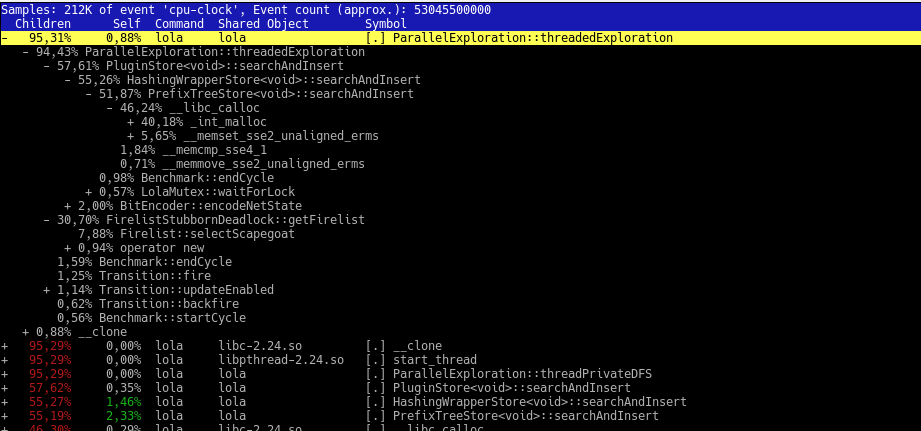
\includegraphics[width=\textwidth]{pictures/perfReportSample.png}
    \caption{perf report output}
    \label{perf_record_sample}
\end{figure}
Figure \ref{perf_record_sample} shows that over 95\% of the samples where taken somewhere in the \texttt{threadedExploration}. This is expected because it is where the search of LoLA is implemented and almost all what LoLA does is searching. We can also see that nearly half of the samples where taken inside the \texttt{searchAndInsert} method of the global store. This observation corresponds to the hint we took from the manual benchmark approach. The two different \texttt{searchAndInsert} methods are caused by the implementation of the \texttt{HashingWrapperStore} which associate each bucket with a \texttt{PrefixTreeStore} and forwards each \texttt{searchAndInsert} to the corresponding \texttt{PrefixTreeStore}.
The new information that we get from the data is that the most samples inside the \texttt{searchAndInsert} methods are taken in a \texttt{\_\_lib\_calloc} call. Almost the half the samples of all taken originate here. They are almost certainly caused by allocating memory on the heap with \texttt{malloc}, \texttt{calloc}, or \texttt{new}. This makes perfect sense, since the perpose of the \texttt{searchAndInsert} method is to store newly discovered net states, which has to be done on the heap. In fact a simplified high level view on the search could be described as:
\begin{enumerate}
    \item Discover a net state
    \item Store the net state
    \item Repeat until all states are discovered
\end{enumerate}
Discovering net states is done by firing a transition from the fire list (a list of al transitions that can be fired from the current net state). Beside the \texttt{searchAndInsert} method we can see this behavior in the profiling data too. Getting the fire list is the second most sampled method inside the \texttt{threadedExploration} and firing the transition was also sampled often enough to account for almost 1\% of all samples.

The calls inside lib calloc are a variety of system calls. Understanding what they really do is outside of the scope of this work. But the last sampled functions containing words like 'lock' or 'wake'. These are probably used to synchronize threads and lock memory regions. Ultimately the allocator has to be thread safe too. Allocating heap space in high frequencies is no common use case, thus the assumption that the allocator just blocks until a request was fully processed seems to be reasonable. Additionally there is only one system allocator for multiple threads. If they all call the same allocator it is likely that they get in each others ways with higher frequent calls and with an increasing amount of used threads.

With perfs data and the previous assumptions we can be quite confident that changing the way we allocate heap space can have an impact on LoLA performance. For example we can reduce the frequent and complex calls to the allocator, by using bigger preallocated chunks of memory (from the system allocator) and manage them by our selfs. This would not only reduce the calls to lib calloc needed, it also has the potential of reducing the overall consumed memory, since we already store pointers to each net state inside the global store. The fact that we store them permanently until LoLA is terminated makes it unnecessary to manage additional data for defragmentation handling. This information can get quite big in the system allocator, especially when allocating a lot of small data like LoLA does. The chunks can also be associated with each thread or each bucket of the \texttt{HashingWrapperStore} to make their access thread safe. This way we can access multiple memory locations by multiple threads. If thread synchronization is really a problem by the system allocator like previously assumed, this potentially resolves the issue of the general sequential performance of LoLA with the parallel implementation.

An implementation for this approach requires a custom allocator that wraps the system calls. Fortunately we have access to exactly such an allocator from a previous project at our chair called 'mara'. The participation of the author of this work at the development of mara is another advantage. The results of this circumstances lead to an integration of mara into LoLA for the net state search.

\section{Allocation strategie change}
In the last chapter we saw that the profiling results lead deeper into the \texttt{searchAndInsert} method. The data suggest that high frequent calls to the system allocator might be the cause of the bottleneck. To see if this assumption is true, we have to change the way LoLA uses the heap und measure the performance again.

We will use the Memory and Resource Allocator (mara) to wrap calls to the system allocator. Mara was previously developed at the chair of theoretical computer science as a student project by Julian Gaede, Marian Stein and Tom Meyer. The later use in LoLA was a part of the project aims.

A major part of maras constraints was that once allocated memory will never be rearranged and never be freed until program termination. Thus it can be freed by the operating system and mara is allowed to drop references that where previously shared. This allows mara to reduce the overhead for heap allocation in space and time.

Mara publishes a class that can be used as a custom allocator. A call to its \texttt{staticNew} method will return a pointer into a previously allocated chunk of memory. The next call to \texttt{staticNew} will return another pointer inside the same chunk that is adjacent to the previously returned memory segment. This memory management is equivalent to a stack. Once the chunk is filled, a new one is allocated with a call to the system allocator. The old chunk is not stored and there is now possibility to access it again with mara (but the previously shared pointers remain valid). Each object of the mara class manages disjoint parts of the heap.

With memory allocated by mara we can very easily distribute LoLAs net state memory to make it thread safe. With the \texttt{HashingWrapperStore} we already have a method to store net states in independent \texttt{PrefixTreeStore}s (inside the buckets). The access to them is already restricted to one thread at a time, while other buckets still can be accessed by other threads. This means that we don not need to consider parallelization issues inside the buckets \texttt{PrefixTreeStore}. All memory access inside can only be done by a single thread. To use mara as allocator, we just have to create one instance of the mara class and substitute all calls to \texttt{malloc}, \texttt{calloc} and \texttt{new} inside the \texttt{PrefixTreeStore} with a call to maras \texttt{staticNew} method. Because calls to delete and free will now produce undefined behavior, these calls have to be removed. The operating system will free the memory on program termination. After that, all heap allocation for the net states is wrapped by mara. 

Altering LoLA in that way we now can start another benchmark to see if the changes impact LoLAs performance.

\section{Results}
\subsection{Profiling}
- same environment like the previous prof env\\
- PIC: data\\
- libcalloc calls are gone -> under significance threshold\\
- mem... calls and fire list calls are now the most significant values\\
- meaning the greatest bottleneck seems to be gone\\

\subsection{Macrobenchmark}
- knowing a major bottleneck is gone, execution and scaling of the whole program is of interest\\
- simple measurement of execution time is sufficient\\
- since multiple threads will influence time consumption directly\\
- lola can log that itself\\
- all implementations are benchmarked (master, CAS, MaraCas, MaraPthread)\\
- significant values are: single thread performance, scaling with threads, scaling with bucket count\\
- PIC: measurements\\

\section{Evaluation}